\section{Artithmetic instructions}

\subsection{Objective}

Write an assembly program to perform the following operations:

\begin{itemize}
    \item[-] Addition
    \item[-] Subtraction
    \item[-] Multiplication
    \item[-] Division
\end{itemize}

\subsection{Implementation}

Using the 8086 microprocessor's instruction set we can perform the above operations.

\subsubsection{Assembly code}

\asmcode{./code/8086/arithmetic_instructions.asm}

\subsection{Output}

\begin{figure}[ht]
    \centering
    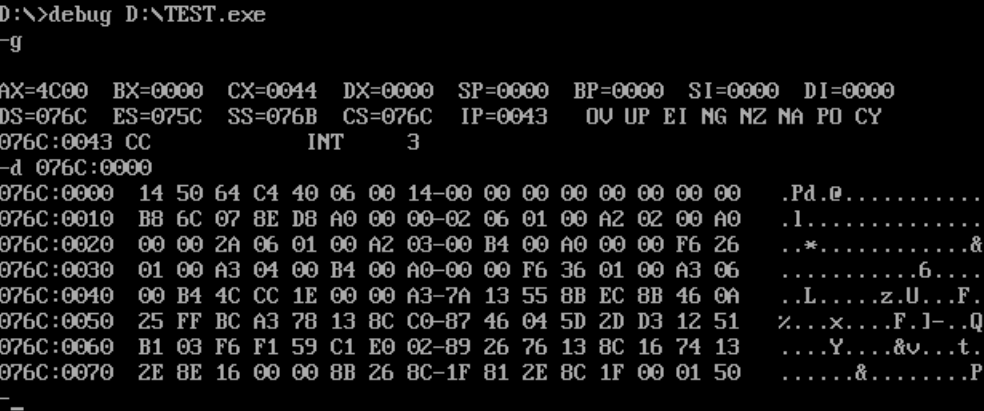
\includegraphics[width=0.8\textwidth]{./res/practicals/arithmetic.png}
    \caption{Output of the program}
    \label{fig:arithmetic_instructions}
\end{figure}

\pagebreak
